\chapter{$bbZZ$ measurements and combination of all HH channels}
\label{ch:bbZZcombination}

Even for the HL-LHC with almost 3\abinv of data, none of the HH analyses can reach the discovery sensitivity, thus the goal for all HH analyses now and in the nearest future is to contribute to the grand combination and only in this collaborative way to achieve the desired sensitivity. From the recent results of the HL-LHC HH combination projection analysis ~\cite{CMS-PAS-FTR-18-019}: "the statistical combination of the five decay channels results in an expected significance for the standard model HH signal of 2.6$\sigma$". This is a clear sign that more data are needed. However, many Higgs analysts would agree that new statistical and MVA tools should be developed/employed. Thus, the next iteration of this analysis will most likely use a sophisticated neural network not only for the signal-background separation, but also for lepton reconstruction, etc. 

This analysis is the search for the double Higgs boson production mediated by the intermediate graviton (and separately) by the radion in the bbZZ channel with the 2 $b$ jets, 2 leptons, 2 neutrinos final state with the $35.9\fbinv$ 2016 dataset. According to the CMS Physics Coordination, for the paper in PRD this analysis has to be combined with the other $bbZZ$ analysis, which is focused on the 2 bjets, 2 leptons, 2 jets signature. %Prior to this $bbZZ$ combination, that each analysis merges the data from both dimuon and dielectron channels. 
The mass range to be covered in the combined measurement is also from 250 GeV to 1000 GeV.

Regarding the latest grand combination for the spin 0 and spin 2 cases ~\cite{CMS-PAS-HIG-17-030} shown at the Fig. \ref{HH_combo}, the results are obtained for the extended mass range going from 250 GeV up to 3000 GeV, but no significant excess is found. The combination is done for the mass regions where at least two decay channels could contribute. Overall, $\bbbar \gamma\gamma$ is the most sensitive channel in the low mass region and $\bbbar \bbbar$ in the higher mass region (above $\sim$500 GeV).

This concludes the discussion of analysis details and in the next chapter we will summarise the main ideas that have been covered throughout this thesis. 


\begin{figure}[H]%hbpt?                                                                       
  \begin{center}
    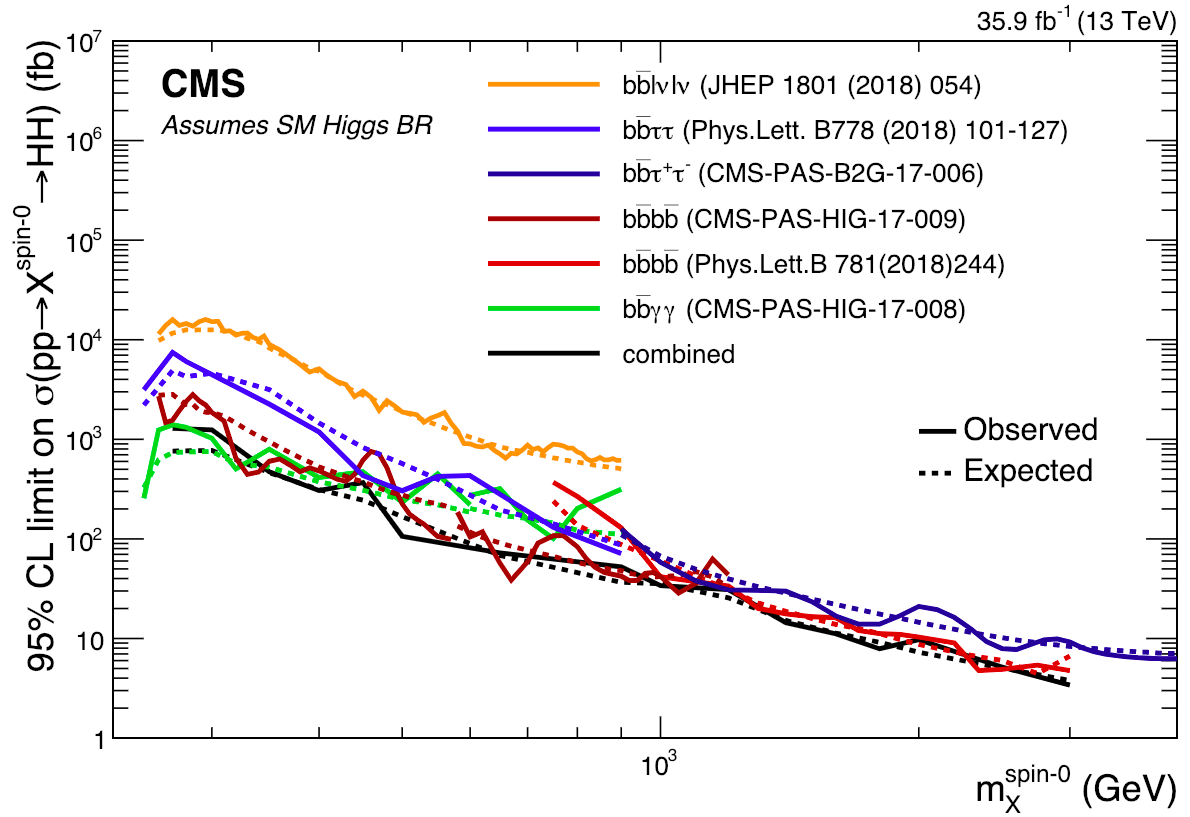
\includegraphics[width=0.65\textwidth]{HH_combo_spin0.png}
    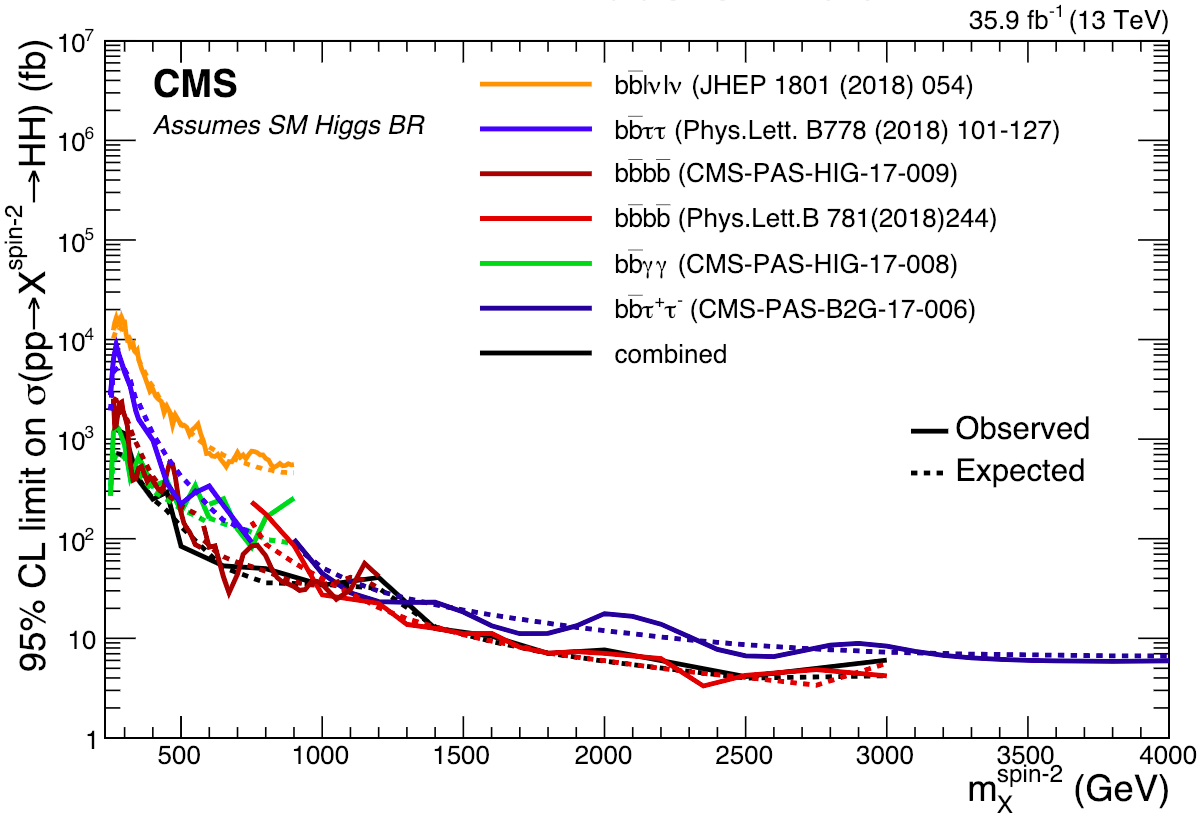
\includegraphics[width=0.65\textwidth]{HH_combo_spin2.png}
    \caption{ Combination of HH channels using 2016 data. Expected (dashed) and observed (solid line) 95\% CL exclusion limits are shown. The results describe the production cross section of a narrow width spin 0 (top) and spin 2 (bottom) resonance decaying into a pair of SM Higgs bosons.  }
    \label{HH_combo}
  \end{center}
\end{figure}





%
%This note presents a search for the production of two Higgs bosons
%through narrow resonances, a KK graviton (spin-2) and a radion (spin-0), where one of the Higgs bosons decays to
%two \Pqb quarks while the other decays to a pair of \PZ bosons which, in
%turn, decay to a pair of neutrinos and a pair of electrons or muons.
%The search is performed with the $35.9\fbinv$ of 2016 data set
%collected by the CMS experiment at the LHC in proton-proton collisions at
%$\sqrt{s} = 13 \TeV$.
%
%No statistically significant deviations from the SM predictions for
%background processes have been observed, and 95\% upper confidence limits are reported for production cross section
%of a KK graviton/radion times the branching fraction of the subsequent decay into an
%HH system. The limits are derived for resonance masses in the 250 GeV to 1 TeV range.
%The limits are set for the mass range of the resonance from 250~GeV to 1~TeV.                                                                                            
%While the computed limits do not lead to exclusion of any resonance mass ranges, when added to other double Higgs decay channels' results from CMS, they will enhance the combined exclusion range.                                                                                                                                               


%The results for the resonant HH production have been presented with                                                                                                      
%the $35.9\fbinv$ of 2016 data set collected from the LHC proton-proton collisions at                                                                                     
%$\sqrt{s} = 13 \TeV$. The results are compatible with the SM within                                                                                                      
%the uncertainties. 95 $\%$ CL upper limits (see Table ~\ref{tab:finalLimits}) are set on the production                                                                  
%of a Higgs boson pair through the intermediate RS KK-graviton in the range of masses from 250 to 1000 GeV.                                                               
%%Interpretation of the model independent results for a narrow spin-2 resonance decaying to a pair of Higgs bosons is done within a WED framework for a graviton particle.                                                                                                                                                                         

